\documentclass[a4paper,11pt]{article}

% Kodovani (cestiny) v dokumentu: utf-8
%\usepackage[cp1250]{inputenc}	% Omezena stredoevropska kodova stranka, pouze MSW.
\usepackage[utf8]{inputenc}	% Doporucujeme pouzivat UTF-8 (unicode).

\usepackage[margin=2cm]{geometry}
\newtoks\jmenopraktika \newtoks\jmeno \newtoks\datum
\newtoks\obor \newtoks\skupina \newtoks\rocnik \newtoks\semestr
\newtoks\cisloulohy \newtoks\jmenoulohy
\newtoks\tlak \newtoks\teplota \newtoks\vlhkost

\jmenopraktika={Fyzikální praktikum 3}
\jmeno={Lukáš Lejdar}
\datum={26. února 2025}
\obor={F}
\skupina={Út 14:00}

\cisloulohy={9}
\jmenoulohy={Studium činnosti fotonásobiče}

\tlak={101{,}35}
\teplota={21,1}
\vlhkost={47,7}


%%%%%%%%%%% Uzitecne balicky:
\usepackage[czech]{babel}

\usepackage{graphicx}
\usepackage{amsmath}
\usepackage{xspace}
\usepackage{url}
\usepackage{indentfirst}
\usepackage{wrapfig}
\usepackage{xcolor}
\usepackage{subfig}
\usepackage{subcaption}
\usepackage{enumitem}
\usepackage{tikzsymbols}
\usepackage{newfloat}

\DeclareFloatingEnvironment[fileext=lof]{graph}
\captionsetup[graph]{labelformat=simple, labelsep=colon, name=Graf}

%%%%%% Zamezeni parchantu:
\widowpenalty 10000 \clubpenalty 10000 \displaywidowpenalty 10000
%%%%%% Parametry pro moznost vsazeni vetsiho poctu obrazku na stranku
\setcounter{topnumber}{3}	  % max. pocet floatu nahore (specifikace t)
\setcounter{bottomnumber}{3}	  % max. pocet floatu dole (specifikace b)
\setcounter{totalnumber}{6}	  % max. pocet floatu na strance celkem
\renewcommand\topfraction{0.9}	  % max podil stranky pro floaty nahore
\renewcommand\bottomfraction{0.9} % max podil stranky pro floaty dole
\renewcommand\textfraction{0.1}	  % min podil stranky, ktery musi obsahovat text
\intextsep=8mm \textfloatsep=8mm  %\intextsep pro ulozeni [h] floatu a \textfloatsep pro [b] or [t]

% Tecky za cisly sekci:
\renewcommand{\thesection}{\arabic{section}.}
\renewcommand{\thesubsection}{\thesection\arabic{subsection}.}
% Jednopismenna mezera mezi cislem a nazvem kapitoly:
\makeatletter \def\@seccntformat#1{\csname the#1\endcsname\hspace{1ex}} \makeatother
%
\newcommand{\vsn}[4]{\ensuremath{#1 =} #2(#3)\,#4}
\newcommand{\vrn}[6]{\ensuremath{#1 =} (#2 $\pm$ #3)\,#4 ($p=$ #5\,\%, $\nu=$ #6)}

\newcommand*\circled[1]{\tikz[baseline=(char.base)]{
		\node[shape=circle,draw,inner sep=1pt] (char) {#1};}}

%%%%%%%%%%%%%%%%%%%%%%%%%%%%%%%%%%%%%%%%%%%%%%%%%%%%%%%%%%%%%%%%%%%%%%%%%%%%%%%
% Zacatek dokumentu
%%%%%%%%%%%%%%%%%%%%%%%%%%%%%%%%%%%%%%%%%%%%%%%%%%%%%%%%%%%%%%%%%%%%%%%%%%%%%%%

\begin{document}

\thispagestyle{empty}

{
\begin{center}
\sf 
{\Large Ústav fyziky a technologií plazmatu Přírodovědecké fakulty Masarykovy univerzity} \\
\bigskip
{\huge \bfseries FYZIKÁLNÍ PRAKTIKUM} \\
\bigskip
{\Large \the\jmenopraktika}
\end{center}

\bigskip

\sf
\noindent
\setlength{\arrayrulewidth}{1pt}
\begin{tabular*}{\textwidth}{@{\extracolsep{\fill}} l l}
\large {\bfseries Zpracoval:}  \the\jmeno & \large  {\bfseries Naměřeno:} \the\datum\\[2mm]
\large  {\bfseries Obor:} \the\obor  \hspace{40mm}  {\bfseries Skupina:} \the\skupina %
&\large {\bfseries Testováno:}\\
\\
\hline
\end{tabular*}
}

\bigskip

{
\sf
\noindent \begin{tabular}{p{4cm} p{0.6\textwidth}}
\Large  Úloha č. {\bfseries \the\cisloulohy:} \par
\smallskip
$T=\the\teplota$~$^\circ$C \par
$p=\the\tlak$~kPa \par
$\varphi=\the\vlhkost$~\%
&\Large \bfseries \the\jmenoulohy  \\[2mm]
\end{tabular}
}

\vskip1cm

\section{Úvod}
 
\section{Postup měření}

\section{Výsledky měření}

\begin{figure}[htpb]
    \centering
    \include{koef_emise_na_energii_el.tex}
    \caption{}
\end{figure}

\begin{figure}[htpb]
    \centering
    % GNUPLOT: LaTeX picture with Postscript
\begingroup
  \makeatletter
  \providecommand\color[2][]{%
    \GenericError{(gnuplot) \space\space\space\@spaces}{%
      Package color not loaded in conjunction with
      terminal option `colourtext'%
    }{See the gnuplot documentation for explanation.%
    }{Either use 'blacktext' in gnuplot or load the package
      color.sty in LaTeX.}%
    \renewcommand\color[2][]{}%
  }%
  \providecommand\includegraphics[2][]{%
    \GenericError{(gnuplot) \space\space\space\@spaces}{%
      Package graphicx or graphics not loaded%
    }{See the gnuplot documentation for explanation.%
    }{The gnuplot epslatex terminal needs graphicx.sty or graphics.sty.}%
    \renewcommand\includegraphics[2][]{}%
  }%
  \providecommand\rotatebox[2]{#2}%
  \@ifundefined{ifGPcolor}{%
    \newif\ifGPcolor
    \GPcolorfalse
  }{}%
  \@ifundefined{ifGPblacktext}{%
    \newif\ifGPblacktext
    \GPblacktexttrue
  }{}%
  % define a \g@addto@macro without @ in the name:
  \let\gplgaddtomacro\g@addto@macro
  % define empty templates for all commands taking text:
  \gdef\gplbacktext{}%
  \gdef\gplfronttext{}%
  \makeatother
  \ifGPblacktext
    % no textcolor at all
    \def\colorrgb#1{}%
    \def\colorgray#1{}%
  \else
    % gray or color?
    \ifGPcolor
      \def\colorrgb#1{\color[rgb]{#1}}%
      \def\colorgray#1{\color[gray]{#1}}%
      \expandafter\def\csname LTw\endcsname{\color{white}}%
      \expandafter\def\csname LTb\endcsname{\color{black}}%
      \expandafter\def\csname LTa\endcsname{\color{black}}%
      \expandafter\def\csname LT0\endcsname{\color[rgb]{1,0,0}}%
      \expandafter\def\csname LT1\endcsname{\color[rgb]{0,1,0}}%
      \expandafter\def\csname LT2\endcsname{\color[rgb]{0,0,1}}%
      \expandafter\def\csname LT3\endcsname{\color[rgb]{1,0,1}}%
      \expandafter\def\csname LT4\endcsname{\color[rgb]{0,1,1}}%
      \expandafter\def\csname LT5\endcsname{\color[rgb]{1,1,0}}%
      \expandafter\def\csname LT6\endcsname{\color[rgb]{0,0,0}}%
      \expandafter\def\csname LT7\endcsname{\color[rgb]{1,0.3,0}}%
      \expandafter\def\csname LT8\endcsname{\color[rgb]{0.5,0.5,0.5}}%
    \else
      % gray
      \def\colorrgb#1{\color{black}}%
      \def\colorgray#1{\color[gray]{#1}}%
      \expandafter\def\csname LTw\endcsname{\color{white}}%
      \expandafter\def\csname LTb\endcsname{\color{black}}%
      \expandafter\def\csname LTa\endcsname{\color{black}}%
      \expandafter\def\csname LT0\endcsname{\color{black}}%
      \expandafter\def\csname LT1\endcsname{\color{black}}%
      \expandafter\def\csname LT2\endcsname{\color{black}}%
      \expandafter\def\csname LT3\endcsname{\color{black}}%
      \expandafter\def\csname LT4\endcsname{\color{black}}%
      \expandafter\def\csname LT5\endcsname{\color{black}}%
      \expandafter\def\csname LT6\endcsname{\color{black}}%
      \expandafter\def\csname LT7\endcsname{\color{black}}%
      \expandafter\def\csname LT8\endcsname{\color{black}}%
    \fi
  \fi
    \setlength{\unitlength}{0.0500bp}%
    \ifx\gptboxheight\undefined%
      \newlength{\gptboxheight}%
      \newlength{\gptboxwidth}%
      \newsavebox{\gptboxtext}%
    \fi%
    \setlength{\fboxrule}{0.5pt}%
    \setlength{\fboxsep}{1pt}%
    \definecolor{tbcol}{rgb}{1,1,1}%
\begin{picture}(5328.00,3600.00)%
    \gplgaddtomacro\gplbacktext{%
      \csname LTb\endcsname%%
      \put(1078,704){\makebox(0,0)[r]{\strut{}$-2.71$}}%
      \put(1078,1038){\makebox(0,0)[r]{\strut{}$-2.7$}}%
      \put(1078,1373){\makebox(0,0)[r]{\strut{}$-2.69$}}%
      \put(1078,1707){\makebox(0,0)[r]{\strut{}$-2.68$}}%
      \put(1078,2041){\makebox(0,0)[r]{\strut{}$-2.67$}}%
      \put(1078,2376){\makebox(0,0)[r]{\strut{}$-2.66$}}%
      \put(1078,2710){\makebox(0,0)[r]{\strut{}$-2.65$}}%
      \put(1078,3045){\makebox(0,0)[r]{\strut{}$-2.64$}}%
      \put(1078,3379){\makebox(0,0)[r]{\strut{}$-2.63$}}%
      \put(1210,484){\makebox(0,0){\strut{}$42$}}%
      \put(1582,484){\makebox(0,0){\strut{}$44$}}%
      \put(1954,484){\makebox(0,0){\strut{}$46$}}%
      \put(2326,484){\makebox(0,0){\strut{}$48$}}%
      \put(2698,484){\makebox(0,0){\strut{}$50$}}%
      \put(3071,484){\makebox(0,0){\strut{}$52$}}%
      \put(3443,484){\makebox(0,0){\strut{}$54$}}%
      \put(3815,484){\makebox(0,0){\strut{}$56$}}%
      \put(4187,484){\makebox(0,0){\strut{}$58$}}%
      \put(4559,484){\makebox(0,0){\strut{}$60$}}%
      \put(4931,484){\makebox(0,0){\strut{}$62$}}%
    }%
    \gplgaddtomacro\gplfronttext{%
      \csname LTb\endcsname%%
      \put(209,2041){\rotatebox{-270}{\makebox(0,0){\strut{} $ I $ ($ \mu A$)}}}%
      \put(3070,154){\makebox(0,0){\strut{}$ U $ ($ V $)}}%
    }%
    \gplbacktext
    \put(0,0){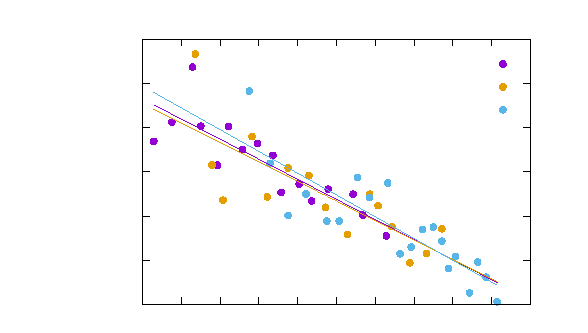
\includegraphics[width={266.40bp},height={180.00bp}]{sigma_na_U}}%
    \gplfronttext
  \end{picture}%
\endgroup

    \caption{}
\end{figure}

\begin{figure}[htpb]
    \centering
    % GNUPLOT: LaTeX picture with Postscript
\begingroup
  \makeatletter
  \providecommand\color[2][]{%
    \GenericError{(gnuplot) \space\space\space\@spaces}{%
      Package color not loaded in conjunction with
      terminal option `colourtext'%
    }{See the gnuplot documentation for explanation.%
    }{Either use 'blacktext' in gnuplot or load the package
      color.sty in LaTeX.}%
    \renewcommand\color[2][]{}%
  }%
  \providecommand\includegraphics[2][]{%
    \GenericError{(gnuplot) \space\space\space\@spaces}{%
      Package graphicx or graphics not loaded%
    }{See the gnuplot documentation for explanation.%
    }{The gnuplot epslatex terminal needs graphicx.sty or graphics.sty.}%
    \renewcommand\includegraphics[2][]{}%
  }%
  \providecommand\rotatebox[2]{#2}%
  \@ifundefined{ifGPcolor}{%
    \newif\ifGPcolor
    \GPcolorfalse
  }{}%
  \@ifundefined{ifGPblacktext}{%
    \newif\ifGPblacktext
    \GPblacktexttrue
  }{}%
  % define a \g@addto@macro without @ in the name:
  \let\gplgaddtomacro\g@addto@macro
  % define empty templates for all commands taking text:
  \gdef\gplbacktext{}%
  \gdef\gplfronttext{}%
  \makeatother
  \ifGPblacktext
    % no textcolor at all
    \def\colorrgb#1{}%
    \def\colorgray#1{}%
  \else
    % gray or color?
    \ifGPcolor
      \def\colorrgb#1{\color[rgb]{#1}}%
      \def\colorgray#1{\color[gray]{#1}}%
      \expandafter\def\csname LTw\endcsname{\color{white}}%
      \expandafter\def\csname LTb\endcsname{\color{black}}%
      \expandafter\def\csname LTa\endcsname{\color{black}}%
      \expandafter\def\csname LT0\endcsname{\color[rgb]{1,0,0}}%
      \expandafter\def\csname LT1\endcsname{\color[rgb]{0,1,0}}%
      \expandafter\def\csname LT2\endcsname{\color[rgb]{0,0,1}}%
      \expandafter\def\csname LT3\endcsname{\color[rgb]{1,0,1}}%
      \expandafter\def\csname LT4\endcsname{\color[rgb]{0,1,1}}%
      \expandafter\def\csname LT5\endcsname{\color[rgb]{1,1,0}}%
      \expandafter\def\csname LT6\endcsname{\color[rgb]{0,0,0}}%
      \expandafter\def\csname LT7\endcsname{\color[rgb]{1,0.3,0}}%
      \expandafter\def\csname LT8\endcsname{\color[rgb]{0.5,0.5,0.5}}%
    \else
      % gray
      \def\colorrgb#1{\color{black}}%
      \def\colorgray#1{\color[gray]{#1}}%
      \expandafter\def\csname LTw\endcsname{\color{white}}%
      \expandafter\def\csname LTb\endcsname{\color{black}}%
      \expandafter\def\csname LTa\endcsname{\color{black}}%
      \expandafter\def\csname LT0\endcsname{\color{black}}%
      \expandafter\def\csname LT1\endcsname{\color{black}}%
      \expandafter\def\csname LT2\endcsname{\color{black}}%
      \expandafter\def\csname LT3\endcsname{\color{black}}%
      \expandafter\def\csname LT4\endcsname{\color{black}}%
      \expandafter\def\csname LT5\endcsname{\color{black}}%
      \expandafter\def\csname LT6\endcsname{\color{black}}%
      \expandafter\def\csname LT7\endcsname{\color{black}}%
      \expandafter\def\csname LT8\endcsname{\color{black}}%
    \fi
  \fi
    \setlength{\unitlength}{0.0500bp}%
    \ifx\gptboxheight\undefined%
      \newlength{\gptboxheight}%
      \newlength{\gptboxwidth}%
      \newsavebox{\gptboxtext}%
    \fi%
    \setlength{\fboxrule}{0.5pt}%
    \setlength{\fboxsep}{1pt}%
    \definecolor{tbcol}{rgb}{1,1,1}%
\begin{picture}(5040.00,3310.00)%
    \gplgaddtomacro\gplbacktext{%
      \csname LTb\endcsname%%
      \put(814,704){\makebox(0,0)[r]{\strut{}$3.1$}}%
      \put(814,1045){\makebox(0,0)[r]{\strut{}$3.2$}}%
      \put(814,1385){\makebox(0,0)[r]{\strut{}$3.3$}}%
      \put(814,1726){\makebox(0,0)[r]{\strut{}$3.4$}}%
      \put(814,2067){\makebox(0,0)[r]{\strut{}$3.5$}}%
      \put(814,2408){\makebox(0,0)[r]{\strut{}$3.6$}}%
      \put(814,2748){\makebox(0,0)[r]{\strut{}$3.7$}}%
      \put(814,3089){\makebox(0,0)[r]{\strut{}$3.8$}}%
      \put(946,484){\makebox(0,0){\strut{}$10$}}%
      \put(1357,484){\makebox(0,0){\strut{}$20$}}%
      \put(1768,484){\makebox(0,0){\strut{}$30$}}%
      \put(2178,484){\makebox(0,0){\strut{}$40$}}%
      \put(2589,484){\makebox(0,0){\strut{}$50$}}%
      \put(3000,484){\makebox(0,0){\strut{}$60$}}%
      \put(3411,484){\makebox(0,0){\strut{}$70$}}%
      \put(3821,484){\makebox(0,0){\strut{}$80$}}%
      \put(4232,484){\makebox(0,0){\strut{}$90$}}%
      \put(4643,484){\makebox(0,0){\strut{}$100$}}%
    }%
    \gplgaddtomacro\gplfronttext{%
      \csname LTb\endcsname%%
      \put(209,1896){\rotatebox{-270}{\makebox(0,0){\strut{}$ \sigma $}}}%
      \put(2794,154){\makebox(0,0){\strut{}$ \Phi $ ($\mu$Lm)}}%
      \csname LTb\endcsname%%
      \put(3933,2025){\makebox(0,0)[r]{\strut{}$U_n = 650$V}}%
      \csname LTb\endcsname%%
      \put(3933,1805){\makebox(0,0)[r]{\strut{}$U_n = 750$V}}%
    }%
    \gplbacktext
    \put(0,0){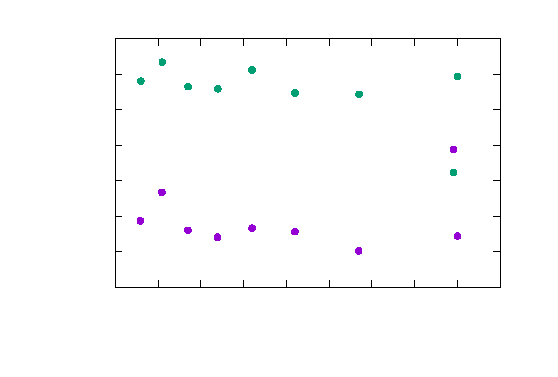
\includegraphics[width={252.00bp},height={165.50bp}]{sigma_na_phi}}%
    \gplfronttext
  \end{picture}%
\endgroup

    \caption{Závislost koeficientu sekundární emise na intenzitě osvětlení fotokatody}
\end{figure} 

\begin{figure}[htpb]
    \centering
    % GNUPLOT: LaTeX picture with Postscript
\begingroup
  \makeatletter
  \providecommand\color[2][]{%
    \GenericError{(gnuplot) \space\space\space\@spaces}{%
      Package color not loaded in conjunction with
      terminal option `colourtext'%
    }{See the gnuplot documentation for explanation.%
    }{Either use 'blacktext' in gnuplot or load the package
      color.sty in LaTeX.}%
    \renewcommand\color[2][]{}%
  }%
  \providecommand\includegraphics[2][]{%
    \GenericError{(gnuplot) \space\space\space\@spaces}{%
      Package graphicx or graphics not loaded%
    }{See the gnuplot documentation for explanation.%
    }{The gnuplot epslatex terminal needs graphicx.sty or graphics.sty.}%
    \renewcommand\includegraphics[2][]{}%
  }%
  \providecommand\rotatebox[2]{#2}%
  \@ifundefined{ifGPcolor}{%
    \newif\ifGPcolor
    \GPcolorfalse
  }{}%
  \@ifundefined{ifGPblacktext}{%
    \newif\ifGPblacktext
    \GPblacktexttrue
  }{}%
  % define a \g@addto@macro without @ in the name:
  \let\gplgaddtomacro\g@addto@macro
  % define empty templates for all commands taking text:
  \gdef\gplbacktext{}%
  \gdef\gplfronttext{}%
  \makeatother
  \ifGPblacktext
    % no textcolor at all
    \def\colorrgb#1{}%
    \def\colorgray#1{}%
  \else
    % gray or color?
    \ifGPcolor
      \def\colorrgb#1{\color[rgb]{#1}}%
      \def\colorgray#1{\color[gray]{#1}}%
      \expandafter\def\csname LTw\endcsname{\color{white}}%
      \expandafter\def\csname LTb\endcsname{\color{black}}%
      \expandafter\def\csname LTa\endcsname{\color{black}}%
      \expandafter\def\csname LT0\endcsname{\color[rgb]{1,0,0}}%
      \expandafter\def\csname LT1\endcsname{\color[rgb]{0,1,0}}%
      \expandafter\def\csname LT2\endcsname{\color[rgb]{0,0,1}}%
      \expandafter\def\csname LT3\endcsname{\color[rgb]{1,0,1}}%
      \expandafter\def\csname LT4\endcsname{\color[rgb]{0,1,1}}%
      \expandafter\def\csname LT5\endcsname{\color[rgb]{1,1,0}}%
      \expandafter\def\csname LT6\endcsname{\color[rgb]{0,0,0}}%
      \expandafter\def\csname LT7\endcsname{\color[rgb]{1,0.3,0}}%
      \expandafter\def\csname LT8\endcsname{\color[rgb]{0.5,0.5,0.5}}%
    \else
      % gray
      \def\colorrgb#1{\color{black}}%
      \def\colorgray#1{\color[gray]{#1}}%
      \expandafter\def\csname LTw\endcsname{\color{white}}%
      \expandafter\def\csname LTb\endcsname{\color{black}}%
      \expandafter\def\csname LTa\endcsname{\color{black}}%
      \expandafter\def\csname LT0\endcsname{\color{black}}%
      \expandafter\def\csname LT1\endcsname{\color{black}}%
      \expandafter\def\csname LT2\endcsname{\color{black}}%
      \expandafter\def\csname LT3\endcsname{\color{black}}%
      \expandafter\def\csname LT4\endcsname{\color{black}}%
      \expandafter\def\csname LT5\endcsname{\color{black}}%
      \expandafter\def\csname LT6\endcsname{\color{black}}%
      \expandafter\def\csname LT7\endcsname{\color{black}}%
      \expandafter\def\csname LT8\endcsname{\color{black}}%
    \fi
  \fi
    \setlength{\unitlength}{0.0500bp}%
    \ifx\gptboxheight\undefined%
      \newlength{\gptboxheight}%
      \newlength{\gptboxwidth}%
      \newsavebox{\gptboxtext}%
    \fi%
    \setlength{\fboxrule}{0.5pt}%
    \setlength{\fboxsep}{1pt}%
    \definecolor{tbcol}{rgb}{1,1,1}%
\begin{picture}(5040.00,2880.00)%
    \gplgaddtomacro\gplbacktext{%
      \csname LTb\endcsname%%
      \put(814,201){\makebox(0,0)[r]{\strut{}$0$}}%
      \put(814,611){\makebox(0,0)[r]{\strut{}$50$}}%
      \put(814,1020){\makebox(0,0)[r]{\strut{}$100$}}%
      \put(814,1430){\makebox(0,0)[r]{\strut{}$150$}}%
      \put(814,1840){\makebox(0,0)[r]{\strut{}$200$}}%
      \put(814,2249){\makebox(0,0)[r]{\strut{}$250$}}%
      \put(814,2659){\makebox(0,0)[r]{\strut{}$300$}}%
      \put(946,-19){\makebox(0,0){\strut{}$550$}}%
      \put(1562,-19){\makebox(0,0){\strut{}$600$}}%
      \put(2178,-19){\makebox(0,0){\strut{}$650$}}%
      \put(2795,-19){\makebox(0,0){\strut{}$700$}}%
      \put(3411,-19){\makebox(0,0){\strut{}$750$}}%
      \put(4027,-19){\makebox(0,0){\strut{}$800$}}%
      \put(4643,-19){\makebox(0,0){\strut{}$850$}}%
    }%
    \gplgaddtomacro\gplfronttext{%
      \csname LTb\endcsname%%
      \put(209,1430){\rotatebox{-270}{\makebox(0,0){\strut{}M $ \cdot 10^6 $ }}}%
      \put(2794,-349){\makebox(0,0){\strut{}$U_n$ (V)}}%
      \csname LTb\endcsname%%
      \put(2134,2486){\makebox(0,0)[r]{\strut{}poloha 1}}%
      \csname LTb\endcsname%%
      \put(2134,2266){\makebox(0,0)[r]{\strut{}poloha 3}}%
      \csname LTb\endcsname%%
      \put(2134,2046){\makebox(0,0)[r]{\strut{}poloha 5}}%
    }%
    \gplbacktext
    \put(0,0){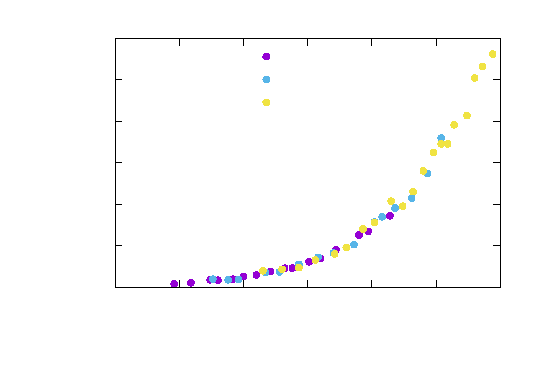
\includegraphics[width={252.00bp},height={144.00bp}]{M}}%
    \gplfronttext
  \end{picture}%
\endgroup

    \caption{}
\end{figure}

\begin{figure}[htpb]
    \centering
    % GNUPLOT: LaTeX picture with Postscript
\begingroup
  \makeatletter
  \providecommand\color[2][]{%
    \GenericError{(gnuplot) \space\space\space\@spaces}{%
      Package color not loaded in conjunction with
      terminal option `colourtext'%
    }{See the gnuplot documentation for explanation.%
    }{Either use 'blacktext' in gnuplot or load the package
      color.sty in LaTeX.}%
    \renewcommand\color[2][]{}%
  }%
  \providecommand\includegraphics[2][]{%
    \GenericError{(gnuplot) \space\space\space\@spaces}{%
      Package graphicx or graphics not loaded%
    }{See the gnuplot documentation for explanation.%
    }{The gnuplot epslatex terminal needs graphicx.sty or graphics.sty.}%
    \renewcommand\includegraphics[2][]{}%
  }%
  \providecommand\rotatebox[2]{#2}%
  \@ifundefined{ifGPcolor}{%
    \newif\ifGPcolor
    \GPcolorfalse
  }{}%
  \@ifundefined{ifGPblacktext}{%
    \newif\ifGPblacktext
    \GPblacktexttrue
  }{}%
  % define a \g@addto@macro without @ in the name:
  \let\gplgaddtomacro\g@addto@macro
  % define empty templates for all commands taking text:
  \gdef\gplbacktext{}%
  \gdef\gplfronttext{}%
  \makeatother
  \ifGPblacktext
    % no textcolor at all
    \def\colorrgb#1{}%
    \def\colorgray#1{}%
  \else
    % gray or color?
    \ifGPcolor
      \def\colorrgb#1{\color[rgb]{#1}}%
      \def\colorgray#1{\color[gray]{#1}}%
      \expandafter\def\csname LTw\endcsname{\color{white}}%
      \expandafter\def\csname LTb\endcsname{\color{black}}%
      \expandafter\def\csname LTa\endcsname{\color{black}}%
      \expandafter\def\csname LT0\endcsname{\color[rgb]{1,0,0}}%
      \expandafter\def\csname LT1\endcsname{\color[rgb]{0,1,0}}%
      \expandafter\def\csname LT2\endcsname{\color[rgb]{0,0,1}}%
      \expandafter\def\csname LT3\endcsname{\color[rgb]{1,0,1}}%
      \expandafter\def\csname LT4\endcsname{\color[rgb]{0,1,1}}%
      \expandafter\def\csname LT5\endcsname{\color[rgb]{1,1,0}}%
      \expandafter\def\csname LT6\endcsname{\color[rgb]{0,0,0}}%
      \expandafter\def\csname LT7\endcsname{\color[rgb]{1,0.3,0}}%
      \expandafter\def\csname LT8\endcsname{\color[rgb]{0.5,0.5,0.5}}%
    \else
      % gray
      \def\colorrgb#1{\color{black}}%
      \def\colorgray#1{\color[gray]{#1}}%
      \expandafter\def\csname LTw\endcsname{\color{white}}%
      \expandafter\def\csname LTb\endcsname{\color{black}}%
      \expandafter\def\csname LTa\endcsname{\color{black}}%
      \expandafter\def\csname LT0\endcsname{\color{black}}%
      \expandafter\def\csname LT1\endcsname{\color{black}}%
      \expandafter\def\csname LT2\endcsname{\color{black}}%
      \expandafter\def\csname LT3\endcsname{\color{black}}%
      \expandafter\def\csname LT4\endcsname{\color{black}}%
      \expandafter\def\csname LT5\endcsname{\color{black}}%
      \expandafter\def\csname LT6\endcsname{\color{black}}%
      \expandafter\def\csname LT7\endcsname{\color{black}}%
      \expandafter\def\csname LT8\endcsname{\color{black}}%
    \fi
  \fi
    \setlength{\unitlength}{0.0500bp}%
    \ifx\gptboxheight\undefined%
      \newlength{\gptboxheight}%
      \newlength{\gptboxwidth}%
      \newsavebox{\gptboxtext}%
    \fi%
    \setlength{\fboxrule}{0.5pt}%
    \setlength{\fboxsep}{1pt}%
    \definecolor{tbcol}{rgb}{1,1,1}%
\begin{picture}(5040.00,3310.00)%
    \gplgaddtomacro\gplbacktext{%
      \csname LTb\endcsname%%
      \put(946,704){\makebox(0,0)[r]{\strut{}$-2.5$}}%
      \put(946,1045){\makebox(0,0)[r]{\strut{}$-2$}}%
      \put(946,1385){\makebox(0,0)[r]{\strut{}$-1.5$}}%
      \put(946,1726){\makebox(0,0)[r]{\strut{}$-1$}}%
      \put(946,2067){\makebox(0,0)[r]{\strut{}$-0.5$}}%
      \put(946,2408){\makebox(0,0)[r]{\strut{}$0$}}%
      \put(946,2748){\makebox(0,0)[r]{\strut{}$0.5$}}%
      \put(946,3089){\makebox(0,0)[r]{\strut{}$1$}}%
      \put(1078,484){\makebox(0,0){\strut{}$550$}}%
      \put(1672,484){\makebox(0,0){\strut{}$600$}}%
      \put(2266,484){\makebox(0,0){\strut{}$650$}}%
      \put(2861,484){\makebox(0,0){\strut{}$700$}}%
      \put(3455,484){\makebox(0,0){\strut{}$750$}}%
      \put(4049,484){\makebox(0,0){\strut{}$800$}}%
      \put(4643,484){\makebox(0,0){\strut{}$850$}}%
    }%
    \gplgaddtomacro\gplfronttext{%
      \csname LTb\endcsname%%
      \put(209,1896){\rotatebox{-270}{\makebox(0,0){\strut{} log($ S $) (A Lm$^{-1} $) }}}%
      \put(2860,154){\makebox(0,0){\strut{}$U_n$ (V)}}%
      \csname LTb\endcsname%%
      \put(2266,2916){\makebox(0,0)[r]{\strut{}poloha 1}}%
      \csname LTb\endcsname%%
      \put(2266,2696){\makebox(0,0)[r]{\strut{}poloha 3}}%
      \csname LTb\endcsname%%
      \put(2266,2476){\makebox(0,0)[r]{\strut{}poloha 5}}%
    }%
    \gplbacktext
    \put(0,0){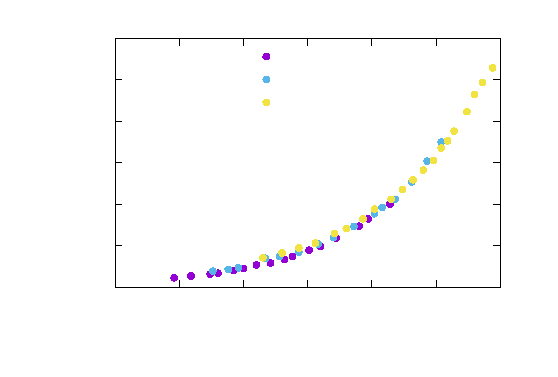
\includegraphics[width={252.00bp},height={165.50bp}]{S}}%
    \gplfronttext
  \end{picture}%
\endgroup

    \caption{}
\end{figure}

\section{Závěr}



\begin{thebibliography}{0}
\bibitem{tabulky} Hustota pevných látek. Dostupné z~\url{http://www.converter.cz/tabulky/hustota-pevne.htmf}.   
\end{thebibliography}

\end{document}
